
%% bare_conf.tex
%% V1.3
%% 2007/01/11
%% by Michael Shell
%% See:
%% http://www.michaelshell.org/
%% for current contact information.
%%
%% This is a skeleton file demonstrating the use of IEEEtran.cls
%% (requires IEEEtran.cls version 1.7 or later) with an IEEE conference paper.
%%
%% Support sites:
%% http://www.michaelshell.org/tex/ieeetran/
%% http://www.ctan.org/tex-archive/macros/latex/contrib/IEEEtran/
%% and
%% http://www.ieee.org/

%%*************************************************************************
%% Legal Notice:
%% This code is offered as-is without any warranty either expressed or
%% implied; without even the implied warranty of MERCHANTABILITY or
%% FITNESS FOR A PARTICULAR PURPOSE!
%% User assumes all risk.
%% In no event shall IEEE or any contributor to this code be liable for
%% any damages or losses, including, but not limited to, incidental,
%% consequential, or any other damages, resulting from the use or misuse
%% of any information contained here.
%%
%% All comments are the opinions of their respective authors and are not
%% necessarily endorsed by the IEEE.
%%
%% This work is distributed under the LaTeX Project Public License (LPPL)
%% ( http://www.latex-project.org/ ) version 1.3, and may be freely used,
%% distributed and modified. A copy of the LPPL, version 1.3, is included
%% in the base LaTeX documentation of all distributions of LaTeX released
%% 2003/12/01 or later.
%% Retain all contribution notices and credits.
%% ** Modified files should be clearly indicated as such, including  **
%% ** renaming them and changing author support contact information. **
%%
%% File list of work: IEEEtran.cls, IEEEtran_HOWTO.pdf, bare_adv.tex,
%%                    bare_conf.tex, bare_jrnl.tex, bare_jrnl_compsoc.tex
%%*************************************************************************

% *** Authors should verify (and, if needed, correct) their LaTeX system  ***
% *** with the testflow diagnostic prior to trusting their LaTeX platform ***
% *** with production work. IEEE's font choices can trigger bugs that do  ***
% *** not appear when using other class files.                            ***
% The testflow support page is at:
% http://www.michaelshell.org/tex/testflow/



% Note that the a4paper option is mainly intended so that authors in
% countries using A4 can easily print to A4 and see how their papers will
% look in print - the typesetting of the document will not typically be
% affected with changes in paper size (but the bottom and side margins will).
% Use the testflow package mentioned above to verify correct handling of
% both paper sizes by the user's LaTeX system.
%
% Also note that the "draftcls" or "draftclsnofoot", not "draft", option
% should be used if it is desired that the figures are to be displayed in
% draft mode.
%
\documentclass[conference]{IEEEtran}
\usepackage{cite}
\usepackage{tipa}
\usepackage{amsmath}%math
\usepackage{amsthm}%proof
\usepackage{xcolor}%color
\usepackage{bm}
\usepackage{graphicx}
\usepackage{booktabs}
\usepackage{textcomp}
\usepackage[colorlinks,linkcolor=black,anchorcolor=black,citecolor=black]{hyperref}
\usepackage{amsfonts,amssymb}
\usepackage{multirow}
\usepackage{float}

\theoremstyle{plain}
\newtheorem{myass}{Assumption}
\newtheorem{mydef}{Definition}
\newtheorem{mylem}{Lemma}
\newtheorem{myrem}{Remark}
\newtheorem{mythm}{Theorem}
% Add the compsoc option for Computer Society conferences.
%
% If IEEEtran.cls has not been installed into the LaTeX system files,
% manually specify the path to it like:
% \documentclass[conference]{../sty/IEEEtran}





% Some very useful LaTeX packages include:
% (uncomment the ones you want to load)


% *** MISC UTILITY PACKAGES ***
%
%\usepackage{ifpdf}
% Heiko Oberdiek's ifpdf.sty is very useful if you need conditional
% compilation based on whether the output is pdf or dvi.
% usage:
% \ifpdf
%   % pdf code
% \else
%   % dvi code
% \fi
% The latest version of ifpdf.sty can be obtained from:
% http://www.ctan.org/tex-archive/macros/latex/contrib/oberdiek/
% Also, note that IEEEtran.cls V1.7 and later provides a builtin
% \ifCLASSINFOpdf conditional that works the same way.
% When switching from latex to pdflatex and vice-versa, the compiler may
% have to be run twice to clear warning/error messages.






% *** CITATION PACKAGES ***
%
%\usepackage{cite}
% cite.sty was written by Donald Arseneau
% V1.6 and later of IEEEtran pre-defines the format of the cite.sty package
% \cite{} output to follow that of IEEE. Loading the cite package will
% result in citation numbers being automatically sorted and properly
% "compressed/ranged". e.g., [1], [9], [2], [7], [5], [6] without using
% cite.sty will become [1], [2], [5]--[7], [9] using cite.sty. cite.sty's
% \cite will automatically add leading space, if needed. Use cite.sty's
% noadjust option (cite.sty V3.8 and later) if you want to turn this off.
% cite.sty is already installed on most LaTeX systems. Be sure and use
% version 4.0 (2003-05-27) and later if using hyperref.sty. cite.sty does
% not currently provide for hyperlinked citations.
% The latest version can be obtained at:
% http://www.ctan.org/tex-archive/macros/latex/contrib/cite/
% The documentation is contained in the cite.sty file itself.






% *** GRAPHICS RELATED PACKAGES ***
%
\ifCLASSINFOpdf
  % \usepackage[pdftex]{graphicx}
  % declare the path(s) where your graphic files are
  % \graphicspath{{../pdf/}{../jpeg/}}
  % and their extensions so you won't have to specify these with
  % every instance of \includegraphics
  % \DeclareGraphicsExtensions{.pdf,.jpeg,.png}
\else
  % or other class option (dvipsone, dvipdf, if not using dvips). graphicx
  % will default to the driver specified in the system graphics.cfg if no
  % driver is specified.
  % \usepackage[dvips]{graphicx}
  % declare the path(s) where your graphic files are
  % \graphicspath{{../eps/}}
  % and their extensions so you won't have to specify these with
  % every instance of \includegraphics
  % \DeclareGraphicsExtensions{.eps}
\fi
% graphicx was written by David Carlisle and Sebastian Rahtz. It is
% required if you want graphics, photos, etc. graphicx.sty is already
% installed on most LaTeX systems. The latest version and documentation can
% be obtained at:
% http://www.ctan.org/tex-archive/macros/latex/required/graphics/
% Another good source of documentation is "Using Imported Graphics in
% LaTeX2e" by Keith Reckdahl which can be found as epslatex.ps or
% epslatex.pdf at: http://www.ctan.org/tex-archive/info/
%
% latex, and pdflatex in dvi mode, support graphics in encapsulated
% postscript (.eps) format. pdflatex in pdf mode supports graphics
% in .pdf, .jpeg, .png and .mps (metapost) formats. Users should ensure
% that all non-photo figures use a vector format (.eps, .pdf, .mps) and
% not a bitmapped formats (.jpeg, .png). IEEE frowns on bitmapped formats
% which can result in "jaggedy"/blurry rendering of lines and letters as
% well as large increases in file sizes.
%
% You can find documentation about the pdfTeX application at:
% http://www.tug.org/applications/pdftex





% *** MATH PACKAGES ***
%
%\usepackage[cmex10]{amsmath}
% A popular package from the American Mathematical Society that provides
% many useful and powerful commands for dealing with mathematics. If using
% it, be sure to load this package with the cmex10 option to ensure that
% only type 1 fonts will utilized at all point sizes. Without this option,
% it is possible that some math symbols, particularly those within
% footnotes, will be rendered in bitmap form which will result in a
% document that can not be IEEE Xplore compliant!
%
% Also, note that the amsmath package sets \interdisplaylinepenalty to 10000
% thus preventing page breaks from occurring within multiline equations. Use:
%\interdisplaylinepenalty=2500
% after loading amsmath to restore such page breaks as IEEEtran.cls normally
% does. amsmath.sty is already installed on most LaTeX systems. The latest
% version and documentation can be obtained at:
% http://www.ctan.org/tex-archive/macros/latex/required/amslatex/math/





% *** SPECIALIZED LIST PACKAGES ***
%
%\usepackage{algorithmic}
% algorithmic.sty was written by Peter Williams and Rogerio Brito.
% This package provides an algorithmic environment fo describing algorithms.
% You can use the algorithmic environment in-text or within a figure
% environment to provide for a floating algorithm. Do NOT use the algorithm
% floating environment provided by algorithm.sty (by the same authors) or
% algorithm2e.sty (by Christophe Fiorio) as IEEE does not use dedicated
% algorithm float types and packages that provide these will not provide
% correct IEEE style captions. The latest version and documentation of
% algorithmic.sty can be obtained at:
% http://www.ctan.org/tex-archive/macros/latex/contrib/algorithms/
% There is also a support site at:
% http://algorithms.berlios.de/index.html
% Also of interest may be the (relatively newer and more customizable)
% algorithmicx.sty package by Szasz Janos:
% http://www.ctan.org/tex-archive/macros/latex/contrib/algorithmicx/




% *** ALIGNMENT PACKAGES ***
%
%\usepackage{array}
% Frank Mittelbach's and David Carlisle's array.sty patches and improves
% the standard LaTeX2e array and tabular environments to provide better
% appearance and additional user controls. As the default LaTeX2e table
% generation code is lacking to the point of almost being broken with
% respect to the quality of the end results, all users are strongly
% advised to use an enhanced (at the very least that provided by array.sty)
% set of table tools. array.sty is already installed on most systems. The
% latest version and documentation can be obtained at:
% http://www.ctan.org/tex-archive/macros/latex/required/tools/


%\usepackage{mdwmath}
%\usepackage{mdwtab}
% Also highly recommended is Mark Wooding's extremely powerful MDW tools,
% especially mdwmath.sty and mdwtab.sty which are used to format equations
% and tables, respectively. The MDWtools set is already installed on most
% LaTeX systems. The lastest version and documentation is available at:
% http://www.ctan.org/tex-archive/macros/latex/contrib/mdwtools/


% IEEEtran contains the IEEEeqnarray family of commands that can be used to
% generate multiline equations as well as matrices, tables, etc., of high
% quality.


%\usepackage{eqparbox}
% Also of notable interest is Scott Pakin's eqparbox package for creating
% (automatically sized) equal width boxes - aka "natural width parboxes".
% Available at:
% http://www.ctan.org/tex-archive/macros/latex/contrib/eqparbox/





% *** SUBFIGURE PACKAGES ***
%\usepackage[tight,footnotesize]{subfigure}
% subfigure.sty was written by Steven Douglas Cochran. This package makes it
% easy to put subfigures in your figures. e.g., "Figure 1a and 1b". For IEEE
% work, it is a good idea to load it with the tight package option to reduce
% the amount of white space around the subfigures. subfigure.sty is already
% installed on most LaTeX systems. The latest version and documentation can
% be obtained at:
% http://www.ctan.org/tex-archive/obsolete/macros/latex/contrib/subfigure/
% subfigure.sty has been superceeded by subfig.sty.



%\usepackage[caption=false]{caption}
%\usepackage[font=footnotesize]{subfig}
% subfig.sty, also written by Steven Douglas Cochran, is the modern
% replacement for subfigure.sty. However, subfig.sty requires and
% automatically loads Axel Sommerfeldt's caption.sty which will override
% IEEEtran.cls handling of captions and this will result in nonIEEE style
% figure/table captions. To prevent this problem, be sure and preload
% caption.sty with its "caption=false" package option. This is will preserve
% IEEEtran.cls handing of captions. Version 1.3 (2005/06/28) and later
% (recommended due to many improvements over 1.2) of subfig.sty supports
% the caption=false option directly:
%\usepackage[caption=false,font=footnotesize]{subfig}
%
% The latest version and documentation can be obtained at:
% http://www.ctan.org/tex-archive/macros/latex/contrib/subfig/
% The latest version and documentation of caption.sty can be obtained at:
% http://www.ctan.org/tex-archive/macros/latex/contrib/caption/




% *** FLOAT PACKAGES ***
%
%\usepackage{fixltx2e}
% fixltx2e, the successor to the earlier fix2col.sty, was written by
% Frank Mittelbach and David Carlisle. This package corrects a few problems
% in the LaTeX2e kernel, the most notable of which is that in current
% LaTeX2e releases, the ordering of single and double column floats is not
% guaranteed to be preserved. Thus, an unpatched LaTeX2e can allow a
% single column figure to be placed prior to an earlier double column
% figure. The latest version and documentation can be found at:
% http://www.ctan.org/tex-archive/macros/latex/base/



%\usepackage{stfloats}
% stfloats.sty was written by Sigitas Tolusis. This package gives LaTeX2e
% the ability to do double column floats at the bottom of the page as well
% as the top. (e.g., "\begin{figure*}[!b]" is not normally possible in
% LaTeX2e). It also provides a command:
%\fnbelowfloat
% to enable the placement of footnotes below bottom floats (the standard
% LaTeX2e kernel puts them above bottom floats). This is an invasive package
% which rewrites many portions of the LaTeX2e float routines. It may not work
% with other packages that modify the LaTeX2e float routines. The latest
% version and documentation can be obtained at:
% http://www.ctan.org/tex-archive/macros/latex/contrib/sttools/
% Documentation is contained in the stfloats.sty comments as well as in the
% presfull.pdf file. Do not use the stfloats baselinefloat ability as IEEE
% does not allow \baselineskip to stretch. Authors submitting work to the
% IEEE should note that IEEE rarely uses double column equations and
% that authors should try to avoid such use. Do not be tempted to use the
% cuted.sty or midfloat.sty packages (also by Sigitas Tolusis) as IEEE does
% not format its papers in such ways.





% *** PDF, URL AND HYPERLINK PACKAGES ***
%
%\usepackage{url}
% url.sty was written by Donald Arseneau. It provides better support for
% handling and breaking URLs. url.sty is already installed on most LaTeX
% systems. The latest version can be obtained at:
% http://www.ctan.org/tex-archive/macros/latex/contrib/misc/
% Read the url.sty source comments for usage information. Basically,
% \url{my_url_here}.





% *** Do not adjust lengths that control margins, column widths, etc. ***
% *** Do not use packages that alter fonts (such as pslatex).         ***
% There should be no need to do such things with IEEEtran.cls V1.6 and later.
% (Unless specifically asked to do so by the journal or conference you plan
% to submit to, of course. )


% correct bad hyphenation here
\hyphenation{op-tical net-works semi-conduc-tor}


\begin{document}
%
% paper title
% can use linebreaks \\ within to get better formatting as desired
\title{Full-order Sliding Mode Control for Deployment/Retrieval of Space Tether System}


% author names and affiliations
% use a multiple column layout for up to three different
% affiliations
\author{\IEEEauthorblockN{Zhiqiang ma}
\IEEEauthorblockA{Research Institute of \\Intelligent Control and Systems\\
Harbin Institute of Technology\\
Harbin, China\\
Email: zhiqiangmahit@gmail.com}
\and
\IEEEauthorblockN{Guanghui Sun}
\IEEEauthorblockA{Research Institute of \\Intelligent Control and Systems\\
Harbin Institute of Technology\\
Harbin, China\\
Email: guanghuisun@hit.edu.cn}
}

% conference papers do not typically use \thanks and this command
% is locked out in conference mode. If really needed, such as for
% the acknowledgment of grants, issue a \IEEEoverridecommandlockouts
% after \documentclass

% for over three affiliations, or if they all won't fit within the width
% of the page, use this alternative format:
%
%\author{\IEEEauthorblockN{Michael Shell\IEEEauthorrefmark{1},
%Homer Simpson\IEEEauthorrefmark{2},
%James Kirk\IEEEauthorrefmark{3},
%Montgomery Scott\IEEEauthorrefmark{3} and
%Eldon Tyrell\IEEEauthorrefmark{4}}
%\IEEEauthorblockA{\IEEEauthorrefmark{1}School of Electrical and Computer Engineering\\
%Georgia Institute of Technology,
%Atlanta, Georgia 30332--0250\\ Email: see http://www.michaelshell.org/contact.html}
%\IEEEauthorblockA{\IEEEauthorrefmark{2}Twentieth Century Fox, Springfield, USA\\
%Email: homer@thesimpsons.com}
%\IEEEauthorblockA{\IEEEauthorrefmark{3}Starfleet Academy, San Francisco, California 96678-2391\\
%Telephone: (800) 555--1212, Fax: (888) 555--1212}
%\IEEEauthorblockA{\IEEEauthorrefmark{4}Tyrell Inc., 123 Replicant Street, Los Angeles, California 90210--4321}}




% use for special paper notices
%\IEEEspecialpapernotice{(Invited Paper)}




% make the title area
\maketitle


\begin{abstract}
%\boldmath
A novel full-order sliding mode tension control scheme for the deployment/retrieval of the space tether system is proposed. The deployment/retrieval dynamics of the space tether system are derived by using Lagrangian mechanics theory. The ideal full-order sliding mode surfaces of the deployment/retrieval dynamics are design using KTC and the second method of Lyapunov, and the designed control technologies can guarantee the asymptotic stability of the full-order sliding mode dynamics. The continuous input is applied to ensure that the system states can reach the ideal surfaces in finite time and keep stable in the subsequent time. The positive tension limit is taken into consideration with choosing appropriate parameters or gains in the design of the full-order sliding mode controller. The numerical results valid the effectiveness of the proposed methods.
\end{abstract}
% IEEEtran.cls defaults to using nonbold math in the Abstract.
% This preserves the distinction between vectors and scalars. However,
% if the conference you are submitting to favors bold math in the abstract,
% then you can use LaTeX's standard command \boldmath at the very start
% of the abstract to achieve this. Many IEEE journals/conferences frown on
% math in the abstract anyway.

% no keywords
\begin{keywords}
Full-order sliding mode; Deployment/retrieval dynamics; Space tether system; Sliding surface design; Tension control;
\end{keywords}




% For peer review papers, you can put extra information on the cover
% page as needed:
% \ifCLASSOPTIONpeerreview
% \begin{center} \bfseries EDICS Category: 3-BBND \end{center}
% \fi
%
% For peerreview papers, this IEEEtran command inserts a page break and
% creates the second title. It will be ignored for other modes.
\IEEEpeerreviewmaketitle



\section{Introduction}
Space tether systems (STS) have been widely used in various space missions, such as the energy collection system~\cite{lanoix2005effect}, deorbiting of the spacecrafts~\cite{khan2014analysis}, the space tug design~\cite{wen2016constrained} and the space elevator application~\cite{kojima2015mission}. Besides the mentioned theory studies, some orbital and suborbital experiments including TSS-1R \cite{lanoix2005effect}, SEDS, YES2~\cite{williams2012review}, have been implemented by space research institutes. The control law design for STS has became important issues and studied by related space research institutes in the recent years~\cite{hallaj2015tethered,alary2015dynamics,wang2015coordinated}. Among the achievements, the deployment/retrieval research has been paid attention to, since it is the fundamental mission for STS~\cite{zhu2015dynamic}.\par
The studies on the deployment/retrival mission of STS have made rapid progress in recent years~\cite{cai2014deployment,ma2014coordinated,jung2015nonlinear,li2016libration}, and many researchers devoted to the deployment/retrival regulation. The presented deployment/retrieval techniques can be classified as the thruster- and the pure tension-control according to the type of the applied actuators. In the former scheme, the thruster is usual applied to regulate the out-of-plane dynamics, i.e., Huang et al. presented the adaptive backstepping method to guarantee the stability of the robot-target combination dynamics, and it was assumed that thrusters provided constant control torque for dynamic stability~\cite{huang2015adaptive}. Mantellato et al. proposed the thruster-aid scheme for the deorbiting device to complete the mission of the debris mitigation~\cite{mantellato2015thrust}. It is  challenging to implement thruster approaches for the deployment/retrieval due to the complicate equipping and the high consumption. Because there exists the difficulties in using thrusters for the mission, researchers have devoted to investigate the tension control methods. In recent years, some meaningful technologies have been achieved, such as the analytical feedback control law~\cite{wen2015space}, the nonlinear dynamic analysis methods~\cite{jung2015nonlinear}, LQG control method~\cite{yousefian2015anti} and the optimal control law~\cite{steindl2015optimal}. The sliding mode control has also been applied for the deployment/retrieval mission, i.e., Liu et al. applied the sliding mode control to stabilize the attitude and the tether length of STS with thruster system. In the mission, thrusters were used to maintain the acceleration of the tether to keep the positive tension~\cite{yingying2012variable}. However, besides the above mentioned technologies, the pure tension sliding mode controller is absent. This is because that there exists some difficulties in designing the control law for deployment/retrieval without thrusters. For example, during the pure tension deployment/retrieval mission, the number of the input for dynamic motion is lower than of the output, hence the system will own the nonlinear underactuated characteristics, and the sliding mode surface is hard to design for nonlinear underactuated systems by using conventional technologies~\cite{edwards2006advances}. In addition, due to the fact that the tension is nonnegative, the designed input is restrict to the positive value~\cite{yingying2012variable}. The mentioned issues make the normal sliding mode technologies no longer have any effect for the deployment/retrieval mission.\par
In this paper, the full-order sliding mode controller (FSMC) is proposed for stabilizing the tether length and the in-plane angle during the deployment/retrieval mission. The linear and nonlinear expressions of the dynamics are both taken into consideration. Referring to the existing analytical technologies~\cite{Vadali1991Feedback}, the full-order sliding mode surface is designed to achieve the asymptotical stability of the dynamics, i.e., a nonlinear sliding mode surface is selected by using the second method of Lyapunov. By choosing the appropriate parameters or gains of the input, the tension can be kept positive. The remainder of the paper is organized as follows. In Section \ref{sec:dynamics}, the deployment/retrieval dynamics are presented, and the full-order siliding-mode control for the linear deployment/retrival dynamics and the related proofs are exhibited in Section \ref{sec:linear control law}. In Section \ref{sec:nonlinear control law} the control law for the nonlinear dynamics is proposed. The numerical simulation is illustrated to validate the control law design.
\section{Dynamics of Space Tether System}\label{sec:dynamics}
The dynamics of STS are shown in Fig \ref{fig:model}The inertial frame is denoted by $OXYZ$, and the origin $O$ locates at center of the frame. $OX$ is on the equatorial plane and pointing towards the spring equinox; $OZ$ is bundling the earth's rotation axis upwards; $OY$ is generated with right-hand rule. The orbital coordinate system is denoted by $O_2xyz$, and $O_2$ locating at the centroid of tether system identifies the origin of the system. $O_2x$ denotes heading of orbital, and $O_2z$ expresses the direction to the earth downwards. $O_2y$ is obtained by using right-hand rule. In addition, $\theta$ and $\phi$ are the symbols of in-plane and the out-of-plane angle. $O_3x'y'z'$ denotes the tether system frame. $O_3z'$ points to the subsatellite along the tether, and $O_3x'$ and $O_3y'$ are generated by rotating STS. One can obtain $O_3x'y'z'$  by the rotation of $O_2xyz$, and $O_3$, $O_2$ are always coincident.\par
\begin{figure}[H]
\centering
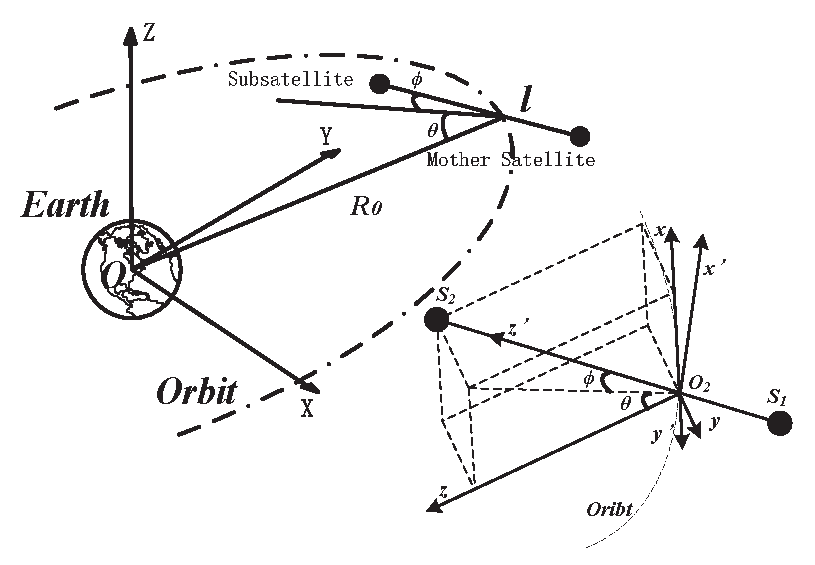
\includegraphics[width=6.68cm,height=4.49cm]{orbit_for_conference.eps}
\caption{Tethered satellite system rigid model}\label{fig:model}
\end{figure}
The symbol system for the STS dynamics will be given as follows. The mass of mother satellite and subsatellite are expressed by $m_1$ and $m_2$ respectively, and the total mass can be described by $m=m_1+m_2$. $\bm{R},\bm{r}$ denote the position vector of the system in relation to $O,O_2$. $\bm{R_0}$ represents the position vector of $O_2$ in relation to $O$. The radius of orbit without any perturbation is expressed by $R_0$; the orbital angular velocity is denoted by $\Omega=\sqrt{\mu_e/R_0^3}$; $\mu_e$ represents the coefficient of the Earth gravity field.\par
It is assumed that the dynamic motion is regarded as a ``ball rolling'', and one can establish a model by using the spherical coordinates to describe the behaviour of STS. It is a fact that the mass of the tether is far less than the one of satellites, hence the mass of the tether is usually ignored. Some other critical assumptions supporting the model analysis follows. The satellites can be treated as particles, since the length of the tether is far greater than the size of the satellites. The ratio of the mass between the two satellites is so tiny that the mother satellite can stay in its nominal orbit by using the station keeping technology, and the motion of the subsatellite won't cause the motion of mother satellite out of control. The gravity forcing on the whole STS should be taken into consideration, and the tether is regard as inextensible, straight and massless. In another words, the tether keeps stiff during the mission.\par
In fact, the out-of-plane motion is coupled with the length of the tether, and in addition, the performance of the in-plane and out-of-plane angle can not be compatible without using the thruster force. The variety range of out-of-plane angle is tiny, when the in-plane plant is controlled stably. The stability of the out-of-plane angle can be guaranteed incidentally with the initial situation satisfying condition $\phi=\dot\phi=0$~\cite{Vadali1991Feedback}.  This paper aims to design control system for the in-plane system, and the out-of-plane plant analysis is ignored here.\par
Considering the assumption of the circular orbit, based on Lagrangian mechanics theory, the kinetic energy and potential energy of the STS can be described by the following forms
\begin{align}
T_t
&= \frac{1}{2}\sum\limits_{s=1}^2 m_s\bm{R_s'\cdot R_s'}\notag\\
&= \frac{1}{2}m\Omega^2R_0^2+\frac{1}{2}\bar{m}l^2(\theta'+\Omega)^2+\frac{1}{2}\bar{m}l'^2\label{eq:Tt1}\\
V_g
&= -\mu_e\sum\limits_{s=1}^2\frac{m_s}{\vert \bm{R_0+r_s}\vert}\notag\\
&= -m\Omega^2R_0^2+\frac{\bar{m}\Omega^2l^2}{2}(1-3cos{^2\theta})\label{eq:Vg}
\end{align}
where $()'$ represents the derivative of $()$, and $l$ is the length of the space tether. $\theta$ is the in-plane angle describing the STS rolling dynamic. For simplifying expression, $\bar{m}$ denotes $m_1m_2/m$; $v_e$ represents the argument of latitude; $\Omega = v_e'$ may be determined under the circular orbit assumption.\par
Combining Eq. (\ref{eq:Tt1}) and (\ref{eq:Vg}), one can obtain $L =T_t-V_g$, and  ${q}=(\theta,l)\in \mathbb{R}^{n\bar{q}}$ identifies the generalized coordinate vector. By utilizing Lagrangian mechanics theory, the dynamics equations hold~\cite{Williams2009745}
\begin{align}
\begin{split}
&\theta''+2(\theta'+\Omega)l'/l+3\Omega^2sin{\theta} cos{\theta}=Q_\theta/(\bar{m}l^2)\\
&\l''-l[(\theta'+\Omega)^2+\Omega^2(3cos{^2\theta}-1)]= -T/\bar{m}\label{eq:motion1}
\end{split}
\end{align}
%% something should be talked about the T
where $T$ is the tension acting on the tether, and the generalized force $Q_\theta$ is related to the in-plane situation. In the pure tension control law, only the tension is existing to control the motion during the deployment/retrieval, and $Q_\theta$ is negligible here. The nondimensional conversion follows for simple expression.
\begin{align}
\lambda=l/L\quad
d()/dt=\Omega d()/dv\quad
\hat{T}=T/(\bar{m}\Omega^2L)\label{eq:varcon}
\end{align}
where the nondimensional tether length satisfies the following condition: $0<\lambda \le 1$; the orbit true anomaly is denoted by $v$; the generalized tension is expressed by $\hat{T}$. $L$ is the total tether length. The length $\lambda$ keeps positive for avoiding the singular dynamics at the beginning of the deployment or the ending of the retrieval, i.e., the desired nondimensional tether length in the deployment can be selected in the region of a small positive value but not zero.\par
Substituting Eq.(\ref{eq:varcon}) into Eq.(\ref{eq:motion1}), one can obtain the nondimension dynamics equations. Since the tether can be deployed to any desired position from an available nonsingular initial one, there exists a variable conversion $\xi =\lambda - a$ where $a\in(0,1]$ representing the desired length of the tether. Select the state vector $\bm{x} = (\theta,\dot\theta,\xi,\dot\xi)^T$, and get
\begin{align}
\begin{cases}
\dot x_1 &= x_2\\
\dot x_2 &= -\frac{2x_4}{x_3+a}(1+x_2)-3\cos{x_1}\sin{x_1}\\
\dot x_3 &= x_3\\
\dot x_4 &= (a+x_3)(1+x_2)^2-(a+x_3)\\&\quad+3(a+x_3)\cos^2{x_1}-\hat{T}.\label{eq:initial system}
\end{cases}
\end{align}
\section{Full-order Sliding Mode Control Law}\label{sec:control law}
In normal sliding mode control scheme, the sliding mode motion is designed as the reduced order system. For some complicated systems, the appropriate reduced sliding mode dynamics are difficult to be select, i.e., it's challenging to choose a ideal sliding mode surface for the deployment/retrieval mission by using the reduced sliding mode dynamics design technology. In addition, the chattering is also a problem to the normal sliding mode control system~\cite{feng2014chattering}. In this section, the full-order sliding mode control scheme is introduced to achieve the the stabilities of the deployment/retrieval dynamics.
\subsection{FSMC for Linear STS}\label{sec:linear control law}
Consider a nominal $n$ order nonlinear system:
\begin{align}
\begin{cases}
\dot{\hat{\bm{x}}} &= \hat{A}\bm{x}\\
\dot x_n &= f(\bm{x},t) + d(\bm{x},t) + b(\bm{x},t)u\label{eq:nominal system}
\end{cases}
\end{align}
where linear matrix $\hat{A}\in R^{(n-1)\times n}$ represents the $n-1$ order system state, and $\bm{x} = [\hat{\bm{x}}^T,x_n]=[x_1,x_2,\ldots,x_n]^T\in R^n$ represents the system state vector, $b(\bm{x},t)$ is invertible, $f(\bm{x},t)$ is nonlinear function, $u\in R$ denotes the system input. The uncertainties and the external disturbance $d(\bm{x},t): R^n\rightarrow R$ is assumed to meet the condition: $d(\bm{x},t)\in L_{\infty}$, i.e., $\sup\limits_{t\ge 0}\vert d(\bm{x},t)\vert\le\alpha<\infty$. A lower number of inputs than degree of freedom (DOF) is the characteristic of underactuated systems in Eq. (\ref{eq:nominal system}), and the following assumptions hold to guarantee the the existence of full-order sliding mode.\par
\begin{myass}
Combine the linear matrix $\hat{A}$ in Eq. (\ref{eq:nominal system}) and auxiliary constant vector $$\hat{\bm{v}} = [a_1,a_2,\ldots,a_{n-1},a_n]^T\in R^n$$ to obtain the full-order system state matrix $A =[\hat{A}^T,\hat{\bm{v}}]^T\in R^{n \times n}$, and the controllability matrix:
$$
M_C = [B\quad AB\quad \ldots\quad A^{n-2}B\quad A^{n-1}B ]
$$
has full rank ($rank M_C = n$).
\end{myass}
\begin{myass}
It is assumed that all state variables are measurable in Eq. (\ref{eq:nominal system}), therefore, the exact values of the functions $f(\bm{x},t)$ and $b(\bm{x},t)$ are all known.
\end{myass}
\begin{myass}
The derivative of external disturbance function with respect to time $\frac{d}{dt}d(\bm{x},t)$ is bounded:
\begin{align}
\vert\frac{d}{dt}d(\bm{x},t)\vert\le \beta \label{eq:dd}
\end{align}
where $\beta$ is a positive constant.
\end{myass}
A full-order sliding mode surface for the system shown in Eq. (\ref{eq:nominal system}) can be established in the following form:
\begin{align}
s&=\dot x_n +\bm{c}^T\bm{x}\notag\\
&= \dot x_n + c_1x_1+c_2x_2+\ldots+c_nx_n\label{eq:slding mode surface 1}
\end{align}
where $c_i(i=1,2,\ldots\,n)$ are undetermined coefficients which will be discussed later. In case that the desired sliding mode satisfying $s = 0$ is present, Eq. (\ref{eq:nominal system}) can be rewrite as follows
\begin{align}
\dot{\bm{x}} = [\hat{A}^T,-\bm{c}]^T\bm{x}.\label{eq:sliding mode system}
\end{align}
According to the Routh-Hurwitz criterion, once the undetermined vector $\bm{c}$ is selected to make the polynomial $p^n+\hat c_np^{n-1}+\ldots+\hat c_2p+\hat c_1$, which corresponds to the system in Eq. (\ref{eq:sliding mode system}), become Hurwitz, the asymptotical stability of the system (\ref{eq:sliding mode system}) can be guaranteed.\par
\begin{mythm}\label{thm:1}
The system shown in Eq. (\ref{eq:nominal system}) will reach the ideal sliding mode surface $s=0$ in finite time and return to the origin asymptotically along $s=0$, if the sliding mode surface is chosen as Eq. (\ref{eq:slding mode surface 1}). The full-order sliding mode control input is proposed in the following form:
\begin{align}
&u = \frac{u_{eq}+u_{sw}}{b(\bm{x},t)}\label{eq:linear u}\\
&u_{eq}=-f(\bm{x,t})-\bm{c}^T\bm{x}\notag\\
&\dot u_{sw}=-\delta u_{sw}-(\beta+\gamma+\eta)sgn(s)\label{eq:solution of u_sw}
\end{align}
where $u_{sw}(0) = 0$; $\bm{c}$ is defined in Eq. (\ref{eq:sliding mode system}); $\eta$ is a positive constant, which will be discussed later; $\delta\ge 0$ and $\gamma\ge\alpha \delta$. The function sgn(s) can be expressed as
\begin{align}
sgn(s)=\begin{cases}
1\quad &s \ge 0\\
-1\quad &s < 0.
\end{cases}\notag
\end{align}
\end{mythm}
\begin{IEEEproof}
Combine the system (\ref{eq:nominal system}) and the sliding mode surface shown in Eq. (\ref{eq:slding mode surface 1}) as follows:
\begin{align}
s   &=\dot x_n +\bm{c}^T\bm{x}\notag\\
    &=f(\bm{x},t)+d(\bm{x,t})+b(\bm{x,t})u+\bm{c}^T\bm{x}.\label{eq:linear sliding mode}
\end{align}\par
Introduce Eq. (\ref{eq:linear u}) into above equation to obtain
\begin{align}
s   &= f(\bm{x},t)+d(\bm{x,t})+u_{eq}+u_{sw}+\bm{c}^T\bm{x}\notag\\
    &= d(\bm{x,t})+u_{sw}.\notag
\end{align}\par
The solution of differential equation (\ref{eq:solution of u_sw}) and the following fundamental relative are given by Feng et al.~\cite{feng2014chattering}
\begin{align}
\begin{split}
u_{sw}(t) = & [u_{sw}(t_0)+(1/\delta)(\beta+\gamma+\eta)sgn(s)]e^{t-t_0}\\
            & -(1/\delta)(\beta+\gamma+\eta)sgn(s)
\end{split}
\end{align}
and
\begin{align}
\gamma\ge\alpha \delta\ge \delta\vert u_{sw}(t)\vert_{max}\ge \delta\vert u_{sw}(t)\vert.\label{eq:beta}
\end{align}\par
The derivative of above equation can be obtained
\begin{align}
\dot s  &= \dot u_{sw}+\frac{d}{dt}d(\bm{x},t)\notag\\
        &= -\delta u_{sw} - (\beta+\gamma+\eta)sgn(s)+\frac{d}{dt}d(\bm{x},t).
\end{align}\par
Select the Lyapunov function candidate $V=\frac{1}{2}s^2$, and its derivative follows
\begin{align}
\dot V  &= s\dot s\notag\\
        &= s(-\delta u_{sw} - (\beta+\gamma+\eta)sgn(s)+\frac{d}{dt}d(\bm{x},t))\notag\\
        &\le \delta\vert u_{sw}\vert\vert s\vert+\vert \frac{d}{dt}d(\bm{x},t))\vert\vert s\vert -(\beta+\gamma+\eta)sgn(s)s.\notag
\end{align}\par
Further substituting Eq. (\ref{eq:beta}) and Eq. (\ref{eq:dd}) into the above equation gives
\begin{align}
\dot V  &\le -\eta\vert s\vert<0 \quad for\quad any\quad s\neq 0
\end{align}
which means that the designed input (\ref{eq:linear u}) will force the sliding mode motion to reach the ideal sliding mode surface in finite time. Once reaching the surface, the behavior of the system (\ref{eq:nominal system}) can be represented by the system shown in Eq. (\ref{eq:sliding mode system}), and with proper coefficients, the system will asymptotically converge to the origin. The proof is completed.
\end{IEEEproof}
Consider linear STS (\ref{eq:initial system}) in the neighbourhood region of the equilibrium showing as follows
\begin{align}
\begin{pmatrix}
\dot x_1\\
\dot x_2\\
\dot x_3\\
\dot x_4
\end{pmatrix}
=
\begin{bmatrix}
0   &1  &0 &0\\
-3  &0  &0 &-2/a\\
0   &0  &0 &1\\
0   &2 &3a &0
\end{bmatrix}
\begin{pmatrix}
x_1\\
x_2\\
x_3\\
x_4
\end{pmatrix}
+
\begin{pmatrix}
0\\0\\0\\3-\hat{T}
\end{pmatrix}.\label{eq:linear mode}
\end{align}\par
By introducing the transform $u_T = 3-\hat T$, the above set of equations can be described by the nominal system (\ref{eq:nominal system}), hence the full-order sliding mode control strategy can be utilized for stabilization. According to the mentioned design procedure, the ideal sliding mode surface should be selected firstly. After choosing a undetermined full-order sliding mode surface
\begin{align}
s_L = \dot x_4 + c_{l1}x_1+c_{l2}x_2+c_{l3}x_3+ c_{l4}x_4\label{eq:linear parameter sliding mode}
\end{align}
for system (\ref{eq:linear mode}), the ideal sliding mode motion on the surface can be described by the following fashion
\begin{align}
\begin{pmatrix}
\dot x_1\\
\dot x_2\\
\dot x_3\\
\dot x_4
\end{pmatrix}
=
\begin{bmatrix}
0   &1  &0 &0\\
-3  &0  &0 &-2/a\\
0   &0  &0 &1\\
-c_{l1}   &2-c_{l2} &3a-c_{l3} &-c_{l4}
\end{bmatrix}
\begin{pmatrix}
x_1\\
x_2\\
x_3\\
x_4
\end{pmatrix}.\label{eq:linear sliding fashion}
\end{align}\par
Coefficients satisfying the tension control conditions and asymptotically stability, will be discussed in Section \ref{sec:numerical simulation}.
\subsection{FSMC for Nonlinear STS}\label{sec:nonlinear control law}
Consider that the $n-1$ order system states are nonlinear in system (\ref{eq:nominal system}):
\begin{align}
\begin{cases}
\dot x_i = f_i(\bm{x},t)\quad i = 1,2,\ldots,n-1\\
\dot x_n = f_n(\bm{x},t)+d'(\bm{x},t)+b'(\bm{x},t)u\label{eq:nonlinear system}
\end{cases}
\end{align}
where $b'(\bm{x},t)\neq 0$ and $f_i(\bm{x},t):R^n\rightarrow R$ are both known nonlinear functions; $d'(\bm{x},t)$ represents the external disturbance. The assumption for $d'(\bm{x},t)$ and $\frac{d}{dt} d'(\bm{x},t)$ is similar to system (\ref{eq:nominal system}):
\begin{align}
\vert d'(\bm{x},t)\vert \le \alpha'\\
\vert \frac{d}{dt} d'(\bm{x},t)\vert \le\beta'.
\end{align}\par
Select the nonlinear sliding mode surface as
\begin{align}
s = \dot x_n + g(\bm{x},t)\label{eq:nonlinear surface}
\end{align}
where nonlinear function $g(\bm{x},t)$ will be discussed later. The system (\ref{eq:nonlinear system}) on the ideal sliding mode surface $s=0$ can be described by
\begin{align}
\dot {\bm{x}} = \hat f(\bm{x},t).\label{eq:dx=fx}
\end{align}\par
If a Lyapunov function candidate can be selected to make system (\ref{eq:dx=fx}) satisfy the asymptotic stability criterion, the system (\ref{eq:nonlinear system}) will asymptotically converge to the origin along the ideal surface $s=0$.
\begin{mythm}\label{eq:thm:2}
For system (\ref{eq:initial system}), a full-order sliding mode surface can be selected as
\begin{align}
s =& \dot x_4+3(x_3+a)+k_1(x_3-x_{3d})-\frac{2k_2x_2}{x_3+a}(x_2+1) \notag\\
&+ k_3x_4- (x_3 +a)[(x_2^2+2x_2+3\cos^2{x_1}]\label{eq:lypunov sliding mode}
\end{align}
where $k_1$, $k_2$, $k_3$ are all positive constants. If the system~(\ref{eq:initial system}) is on the above sliding mode surface $s=0$, the state will converge asymptotically to the equilibrium $\bm{x}_d=(0,0,x_{3d},0)^T$.
\end{mythm}
\begin{IEEEproof}
If the system (\ref{eq:initial system}) is on the above sliding mode surface $s=0$, the following equations hold
\begin{align}
\begin{cases}
\dot x_1 =& x_2\\
\dot x_2 =& -\frac{2x_4}{x_3+a}(1+x_2)-3\cos{x_1}\sin{x_1}\\
\dot x_3 =& x_3\\
\dot x_4 =& -3(x_3+a)+k_1(x_3-x_{3d})-\frac{2k_2x_2x_4}{x_3+a}(x_2+1)\\
&+ k_3x_4+ (x_3 +a)[(x_2^2+2x_2+3\cos^2{x_1}].
\end{cases}\label{eq:lypunov state}
\end{align}\par
Select a Lyapunov function candidate which owns some similarities to that mentioned by Vadali et al.~\cite{Vadali1991Feedback1}.
\begin{align}
V =& \frac{1}{2}[x_4^2+k_1(x_3-x_{3d})^2\notag\\
&+[k_2+(x_3+a)^2](x_2^2+3\sin^2 x_1)].
\end{align}\par
The derivative of the Lyapunov function follows
\begin{align}
\dot V= & x_4\dot x_4+k_1x_4(x_3-x_{3d})+k_2x_2\dot x_2+3k_2x_2\sin x_1\cos x_1\notag\\
        & +x_4x_2^2(x_3+a)+3x_4(x_3+a)\sin^2 x_1 \notag\\&+ \dot x_2x_2(x_3+a)^2 + 3x_2(x_3+a)^2\sin x_1\cos x_1.\notag
\end{align}\par
Substituting Eq. (\ref{eq:lypunov state}) into above equation holds
\begin{align}
\dot V= -k_3x_4^2 < 0\quad for\quad x_4\neq 0
\end{align}
which means the state on the ideal sliding mode surface will converge asymptotically to the equilibrium.\par
The proof is completed.
\end{IEEEproof}
\begin{mythm}\label{thm:3}
The system state shown in Eq. (\ref{eq:initial system}) will reach the ideal sliding mode surface $s=0$ in finite time and return to the origin asymptotically along $s=0$, if the sliding mode surface is chosen as Eq. (\ref{eq:lypunov sliding mode}) and the full-order sliding mode control input is proposed in the following form:
\begin{align}
u =& \frac{u_{eq}+u_{sw}}{b(\bm{x},t)}- k_3x_4\notag\\
u_{eq}=&-f(\bm{x,t})-3(x_3+a)-k_1(x_3-x_{3d}) \notag\\
&+ (x_3 +a)[(x_2^2+2x_2+3\cos^2{x_1}]\notag\\
&+\frac{2k_2x_2}{x_3+a}(x_2+1)\notag\\
\dot u_{sw}=&-\delta u_{sw}-(\beta'+\gamma'+\eta')sgn(s)\notag
\end{align}
where $u_{sw}(0) = 0$; $\bm{c}$ is defined in Eq. (\ref{eq:sliding mode system}); $\eta'$ is a positive constant; $\gamma'\ge\alpha' \delta$.
\end{mythm}
\begin{IEEEproof}
The proof is similar to Theorem \ref{thm:1} and omitted here.
\end{IEEEproof}
\section{Numerical Simulation}\label{sec:numerical simulation}
In order to verify the effectiveness of the proposed full-order sliding mode control schemes in Section \ref{sec:control law}, numerical simulations are going to be implemented in the following.\par
During the simulation, all of the parameters refer to the project YES2. The total length of the tether is 3.5 km, which means that the length of the initial condition of retrieval (the final condition of deployment) for STS is 3.5 km, and it is assumed that the distance between two satellites remains 70 m at least for avoiding singularity. The STS orbits at the altitude of 260 km, and it is assumed that the initial anomaly is 0 degrees. Some physical characteristics of STS in project YES2 are listed as follows: the mass of the mother satellite is 6530 kg, and the mass of the subsatellite is 12 kg. At last but not least, according to the previous researches, in the low orbit altitude, the main perturbations are the solar radiation pressure torque and the aerodynamic torque, and the values of the perturbations are both in the range around $1e^{-5}$ Nm.\par
The parameters or gains are important parts of the control schemes proposed in Section \ref{sec:control law}. The details of the parameters are exhibited in the following. For linear system (\ref{eq:linear sliding fashion}), the parameter of the transform $\xi = \lambda - a$ can be selected as $a=1$, hence the boundary conditions are determined for the deployment/retrieval of STS, i.e. $\bm{x}_0=(0,0,-0.98,0.5)$ and $\bm{x}_d=(0,0,0,0)$ respectively in the mission of the deployment. Besides guaranteeing the stability of the system, the gains or parameters should be selected to keep the tension positive. For the linear STS (\ref{eq:linear mode}), the parameters of the sliding mode surface (\ref{eq:linear parameter sliding mode}) can be determined by using Kelvin-Tait-Chetaev (KTC) theorem~\cite{sun2014fractional}: $c_{l1}=0$, $c_{l2}=-2$, $c_{l3}=0.6$ and $c_{l4}=2$. For the nonlinear STS (\ref{eq:dx=fx}), the parameters of the sliding mode surface (\ref{eq:lypunov sliding mode}) can be selected by using the second method of Lyapunov~\cite{Vadali1991Feedback}, i.e., for the retrieval mission $k_1=1$, $k_2=0$ and $k_3=3$. For the deployment mission, the low gain $k_1=0.016$ has to be chosen to satisfy the limit of the tension control, which makes the response of the tether length become slow obviously. The parameters of the input are listed as follosw: $\delta = 0.1$, $\alpha=\beta=\alpha'=\beta'=2$, $\gamma=\gamma'=2$ and $\eta=\eta'=6$.\par
\begin{figure}
\centering
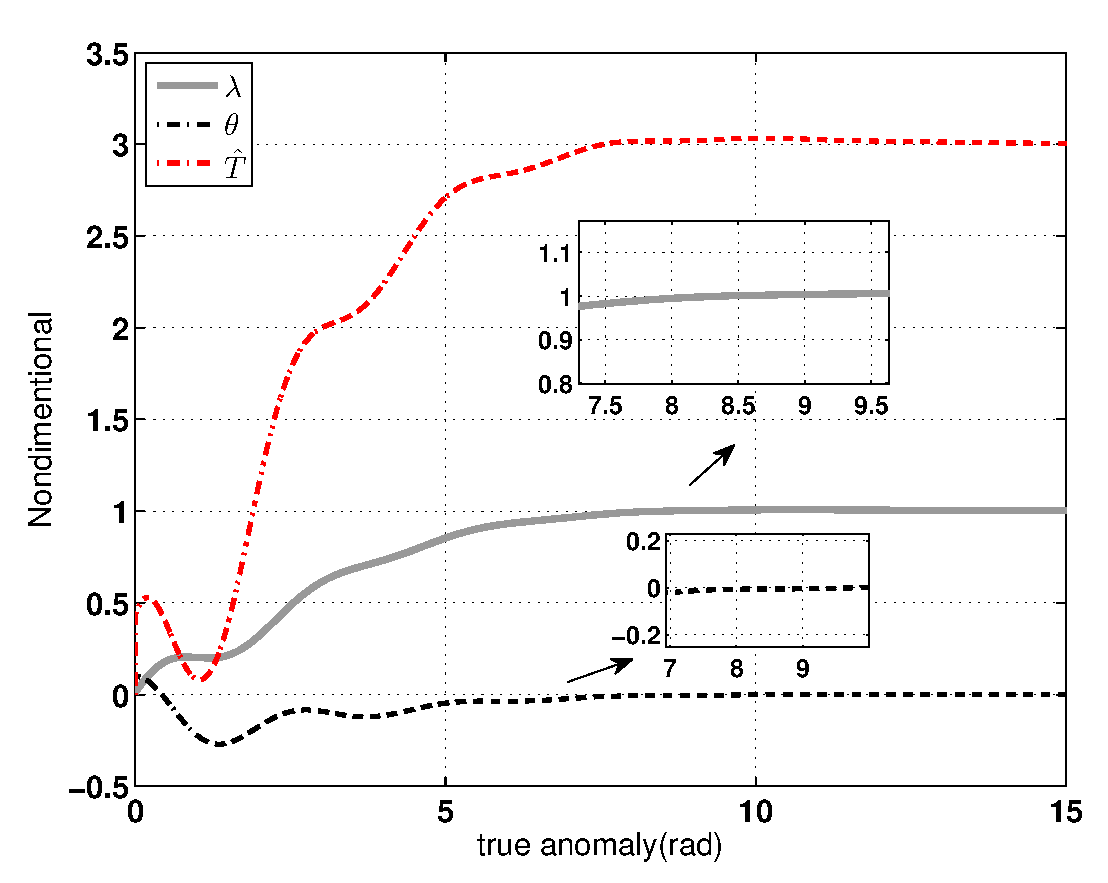
\includegraphics[width=180pt,height=144pt]{linear_deployment.eps}
\caption{Deployment of linearization: length, in-plane angle and tension}
\label{fig:Deployment of linearization}
\end{figure}
The simulation results of the linear STS using full-order sliding mode are shown in Fig \ref{fig:Deployment of linearization} and Fig \ref{fig:Retrieval of linearization}. Fig \ref{fig:Deployment of linearization} shows that the length is deployed from 0.02 of the nondimentional length to 1 at about 8.5 rads, and then the length stays in the subsequent time. During the deployment, the variety of the in-plane angle is in a reasonable range $[-0.27, 0.1]$ rads. It is observed that the tension is positive during the deployment process, which satisfies the requirement of the realistic application. Figure \ref{fig:Retrieval of linearization} shows that the process of the retrieval has an excellent performance, and all of the related states converge to the desired states at about 9 rads.\par
\begin{figure}
\centering
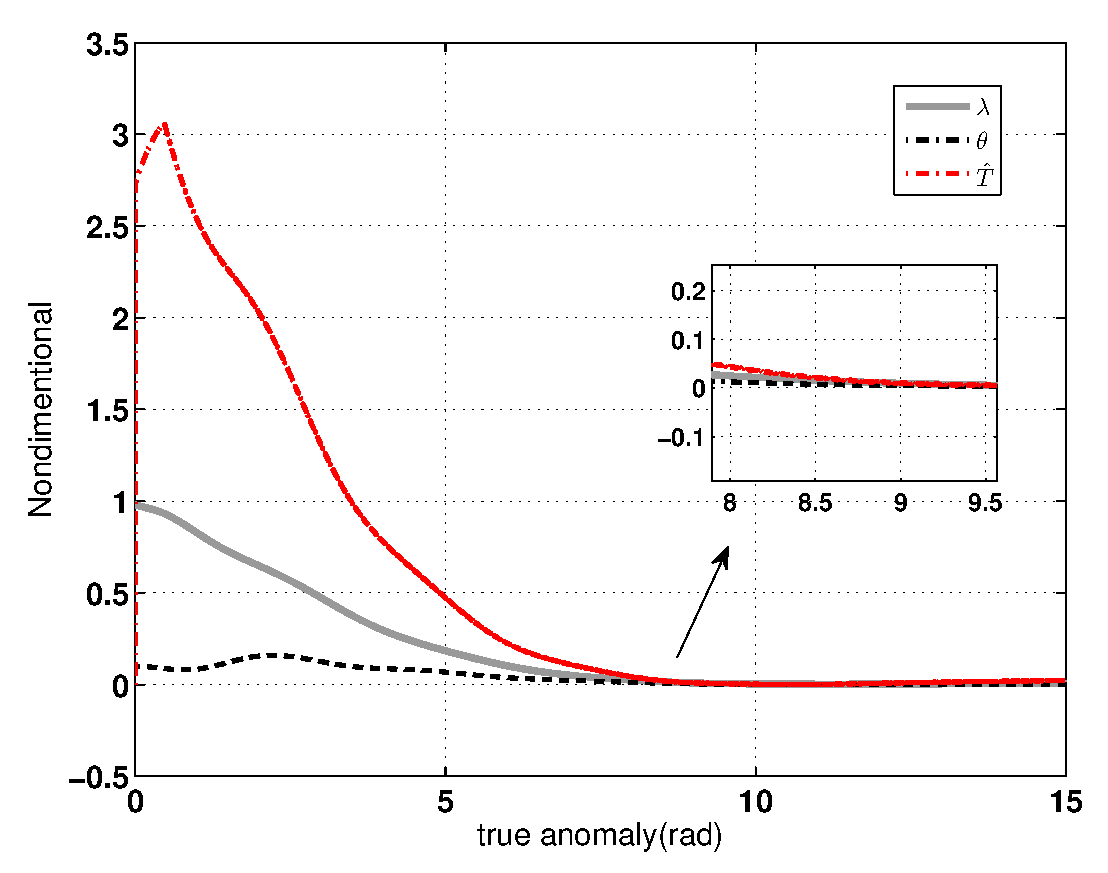
\includegraphics[width=180pt,height=144pt]{linear_retrieval.eps}
\caption{Retrieval of linearization: length, in-plane angle and tension}
\label{fig:Retrieval of linearization}
\end{figure}
Fig \ref{fig:Retrieval of nonlinearization} exhibits the simulation results of the retrieval mission of the nonlinear STS. It is obvious that the process of the retrieval is more direct than the deployment. The nondimentional length and in-plane angle both return to the origin at about 10 rads, and the tension is regulated to stay positive by using the full-order sliding mode control scheme.\par
For the deployment mission of the nonlinear STS, the states of the nondimentional length and the in-plane angle are shown in Fig \ref{fig:Deployment of nonlinearization}, and it is observed that both of the states return to the neighbour range of the origin at about 10.5 rads directly. The variety of the in-plane angle locate in $[0, 0.45]$ rads. The controlling performance satisfies the practical requirement, although the range is larger than the linear one.\par
\begin{figure}
\centering
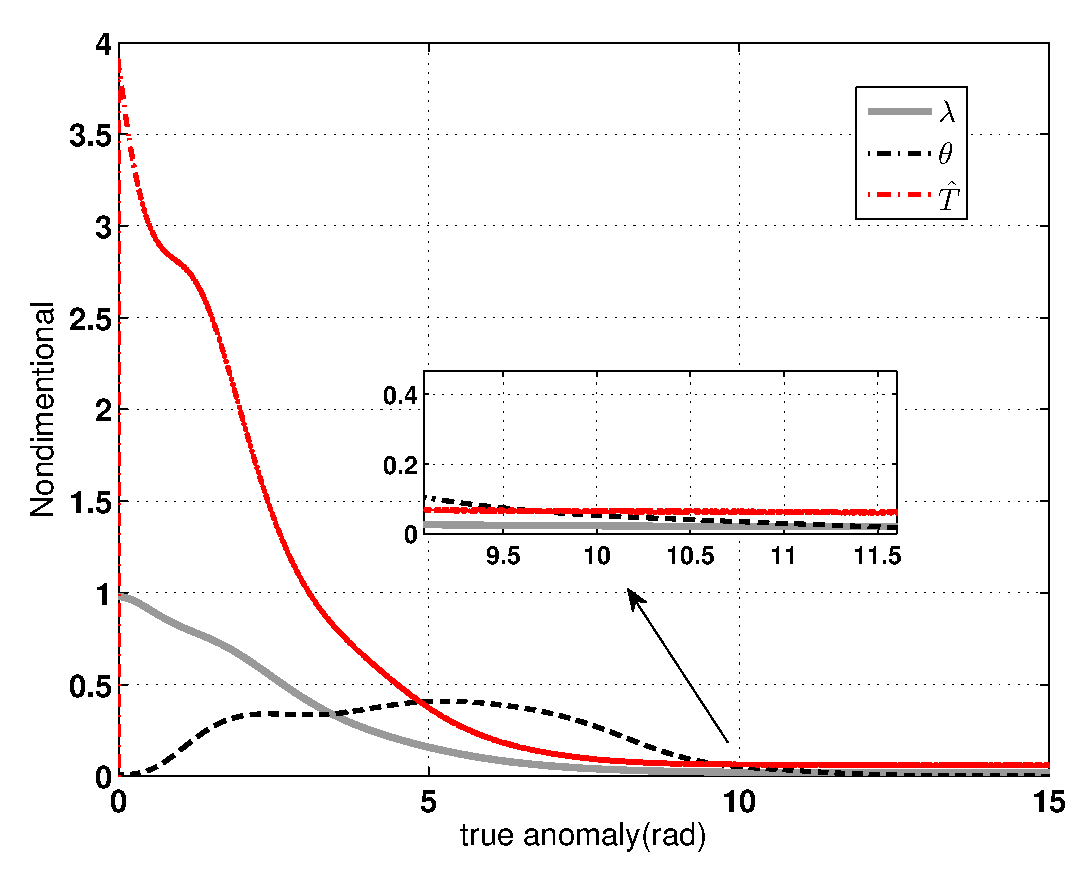
\includegraphics[width=180pt,height=144pt]{lyapunov_retrieval.eps}
\caption{Retrieval of nonlinear STS: length, in-plane angle and tension}
\label{fig:Retrieval of nonlinearization}
\end{figure}
\begin{figure}
\centering
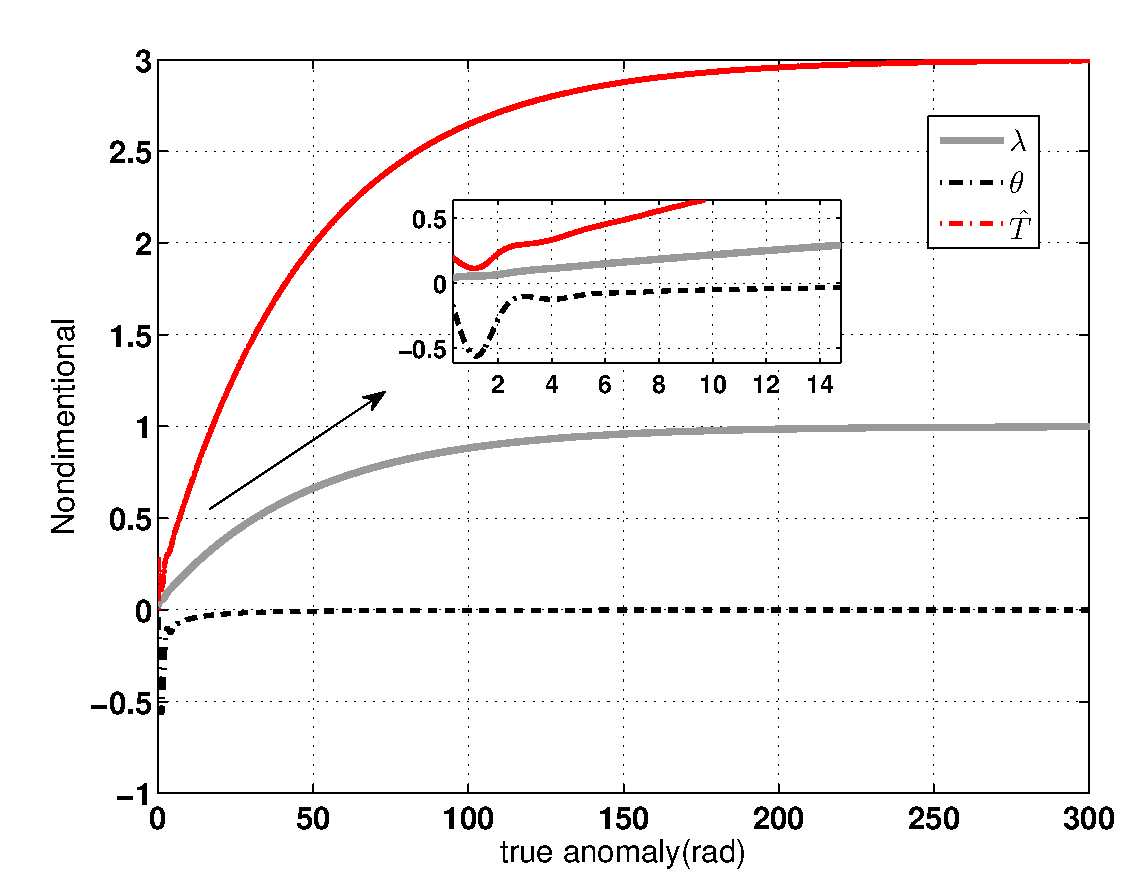
\includegraphics[width=180pt,height=144pt]{lyapunov_deployment.eps}
\caption{Deployment of nonlinear STS: length, in-plane angle and tension}
\label{fig:Deployment of nonlinearization}
\end{figure}
A slow response of the length for the nonlinear STS is shown in Figure \ref{fig:Deployment of nonlinearization}, since the low gains have to be selected for guaranteeing the positive tension. It is observed that the deployment process lasts a long time, and all the tether is deployed at about 270 rads.
\section{Conclusion}
In this paper, the full-order sliding mode control scheme has been proposed for regulating the in-plane deployment/retrival dynamics of STS. Considering the limit of the positive tension, the ideal sliding mode surfaces have been designed to guarantee the asymptotically stability of the full-order sliding mode dynamics, and the parameters of the surfaces can be selected by using the existing analytical stability technology. In addition, applying the continuous input has reduced the chattering in some extent. The full-order sliding mode controller can achieve the reasonable performance for the deployment/retrival mission of STS, and furthermore, the design technology of the full-order sliding mode control can be applied on underactuated systems whose asymptotically stability has been verified by analytical methods.

% An example of a floating figure using the graphicx package.
% Note that \label must occur AFTER (or within) \caption.
% For figures, \caption should occur after the \includegraphics.
% Note that IEEEtran v1.7 and later has special internal code that
% is designed to preserve the operation of \label within \caption
% even when the captionsoff option is in effect. However, because
% of issues like this, it may be the safest practice to put all your
% \label just after \caption rather than within \caption{}.
%
% Reminder: the "draftcls" or "draftclsnofoot", not "draft", class
% option should be used if it is desired that the figures are to be
% displayed while in draft mode.
%
%\begin{figure}[!t]
%\centering
%\includegraphics[width=2.5in]{myfigure}
% where an .eps filename suffix will be assumed under latex,
% and a .pdf suffix will be assumed for pdflatex; or what has been declared
% via \DeclareGraphicsExtensions.
%\caption{Simulation Results}
%\label{fig_sim}
%\end{figure}

% Note that IEEE typically puts floats only at the top, even when this
% results in a large percentage of a column being occupied by floats.


% An example of a double column floating figure using two subfigures.
% (The subfig.sty package must be loaded for this to work.)
% The subfigure \label commands are set within each subfloat command, the
% \label for the overall figure must come after \caption.
% \hfil must be used as a separator to get equal spacing.
% The subfigure.sty package works much the same way, except \subfigure is
% used instead of \subfloat.
%
%\begin{figure*}[!t]
%\centerline{\subfloat[Case I]\includegraphics[width=2.5in]{subfigcase1}%
%\label{fig_first_case}}
%\hfil
%\subfloat[Case II]{\includegraphics[width=2.5in]{subfigcase2}%
%\label{fig_second_case}}}
%\caption{Simulation results}
%\label{fig_sim}
%\end{figure*}
%
% Note that often IEEE papers with subfigures do not employ subfigure
% captions (using the optional argument to \subfloat), but instead will
% reference/describe all of them (a), (b), etc., within the main caption.


% An example of a floating table. Note that, for IEEE style tables, the
% \caption command should come BEFORE the table. Table text will default to
% \footnotesize as IEEE normally uses this smaller font for tables.
% The \label must come after \caption as always.
%
%\begin{table}[!t]
%% increase table row spacing, adjust to taste
%\renewcommand{\arraystretch}{1.3}
% if using array.sty, it might be a good idea to tweak the value of
% \extrarowheight as needed to properly center the text within the cells
%\caption{An Example of a Table}
%\label{table_example}
%\centering
%% Some packages, such as MDW tools, offer better commands for making tables
%% than the plain LaTeX2e tabular which is used here.
%\begin{tabular}{|c||c|}
%\hline
%One & Two\\
%\hline
%Three & Four\\
%\hline
%\end{tabular}
%\end{table}


% Note that IEEE does not put floats in the very first column - or typically
% anywhere on the first page for that matter. Also, in-text middle ("here")
% positioning is not used. Most IEEE journals/conferences use top floats
% exclusively. Note that, LaTeX2e, unlike IEEE journals/conferences, places
% footnotes above bottom floats. This can be corrected via the \fnbelowfloat
% command of the stfloats package.







% conference papers do not normally have an appendix


% use section* for acknowledgement





% trigger a \newpage just before the given reference
% number - used to balance the columns on the last page
% adjust value as needed - may need to be readjusted if
% the document is modified later
%\IEEEtriggeratref{8}
% The "triggered" command can be changed if desired:
%\IEEEtriggercmd{\enlargethispage{-5in}}

% references section

% can use a bibliography generated by BibTeX as a .bbl file
% BibTeX documentation can be easily obtained at:
% http://www.ctan.org/tex-archive/biblio/bibtex/contrib/doc/
% The IEEEtran BibTeX style support page is at:
% http://www.michaelshell.org/tex/ieeetran/bibtex/
%\bibliographystyle{IEEEtran}
% argument is your BibTeX string definitions and bibliography database(s)
%\bibliography{IEEEabrv,../bib/paper}
\section{Acknowledgment}
This work is partially supported by the National Natural Science Foundation of China (No. 61104112, 61503097).
\bibliography{refdatabase}
\bibliographystyle{IEEEtran}
% <OR> manually copy in the resultant .bbl file
% set second argument of \begin to the number of references
% (used to reserve space for the reference number labels box)


% that's all folks
\end{document}


